\section{Injections}
\label{sec:intro_injections}

You may now wonder how you are supposed to solve certain other problems like string manipulation. In this chapter you will learn how to implement methods that you cannot express as SDMs by adding handwritten code to classes, which are created from your model.

Injections are the preferred way to do this by creating partial classes in a small DSL. This approach is inspired by the partial classes in C\# and leads to a clean separation of generated and handwritten code.

There are two ways of adding your code to the generated classes:

\begin{enumerate}
    \item Add code to functions that already exist in the model. This might be necessary, if you can define the header of the function in your model, but the body is too complex to express it as a SDM.
    \item Add own functions and member variables to a class, e.g. to structure your code in private methods.
\end{enumerate}

\subsection{Add card content to the string representation of your box}

\begin{enumerate}
    \item[$\blacktriangleright$] In order to implement \texttt{Box::addToStringRep} right-click on your class \texttt{Box} in Eclipse and choose ``eMoflon$\rightarrow$Create injection for class'' (Fig.~\ref{fig:injection_create_injection}).

    \begin{figure}[htbp]
        \centering
        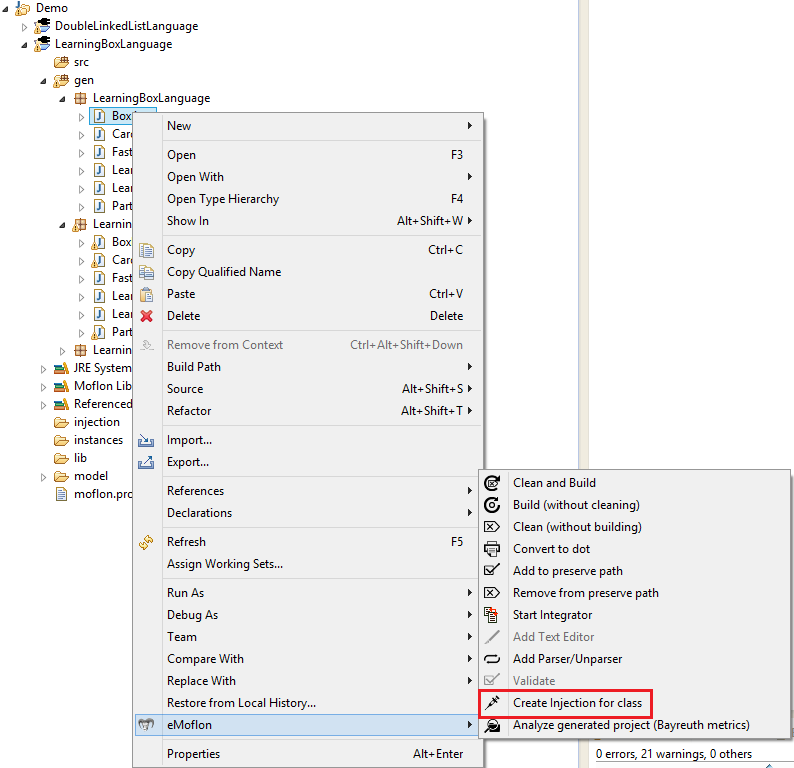
\includegraphics[width=\textwidth]{pics/injectionBilder/create_injection_context_menu.png}
        \caption{Create a new injection}
        \label{fig:injection_create_injection}
    \end{figure}

    This creates you a new file in the ''injection'' folder of your project with the same packages and name as the class but ''.inject'' as extension (Fig. \ref{fig:injection_created_injection_file}). This file contains the definition of a \textit{partial class} similar a normal class in Java (Fig. \ref{code:empty_inject_file}). 

    \begin{figure}[htbp]
        \centering
        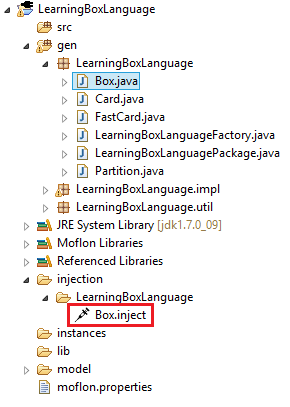
\includegraphics[width=0.6\textwidth]{pics/injectionBilder/newly_created_injection_file.png}
        \caption{Create a new injection}
        \label{fig:injection_created_injection_file}
    \end{figure}
    \FloatBarrier

    \lstdefinelanguage{Injection}[]{Java}{
        morekeywords={partial, class},
        sensitive=false,
        keywordstyle={\bfseries\color{purple}},
        emph={@model},
        emphstyle={\color{blue}},
        backgroundcolor=\color{white}
    }

    \begin{figure}[htbp]
        \centering
        \begin{lstlisting}[language=Injection]
            partial class Box
            {

            }
        \end{lstlisting}
        \caption{Empty injection}
        \label{code:empty_inject_file}
    \end{figure}
    \FloatBarrier

    \item[$\blacktriangleright$]In order to implement \texttt{Box::addToStringRep}, insert the code given in Fig. \ref{code:complete_inject_file} into your injection file. You can use Eclipse templates by entering an ''@'' and pressing ''ctrl+space''.

    \begin{figure}[htbp]
        \centering
        \begin{lstlisting}[language=Injection]
            partial class Box
            {
                @model addToStringRep(Card card) <--
                    StringBuilder sb = new StringBuilder();
                    if (stringRep == null)
                    {
                        sb.append("BoxContent: [");
                    }
                    else
                    {
                        sb.append(stringRep);
                        sb.append(", [");
                    }
                    sb.append(card.getFace());
                    sb.append(", ");
                    sb.append(card.getBack());
                    sb.append("]");
                    stringRep = sb.toString();
                -->
            }
        \end{lstlisting}
        \caption{Complete injection}
        \label{code:complete_inject_file}
    \end{figure}
    \FloatBarrier
    \item[$\blacktriangleright$] Now you can rebuild your project (right-click on ''LearningBoxLanguage'' and choose ''eMoflon $\rightarrow$ Clean and build'') and your code will appear in ''LearningBoxLanguage.impl.BoxImpl'' (Fig. \ref{fig:injected_code_in_boxImpl}). For more information about injections, read appendix \ref{sec:appendix_injections}.

\end{enumerate}

    

    \begin{figure}[htbp]
        \centering
        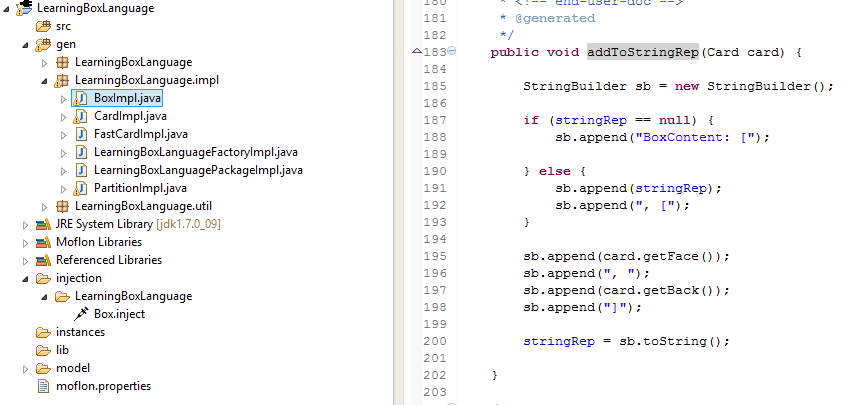
\includegraphics[width=\textwidth]{pics/injectionBilder/injected_code_in_impl.png}
        \caption{Injected code in BoxImpl}
        \label{fig:injected_code_in_boxImpl}
    \end{figure}